\documentclass[12pt]{article}
\usepackage{geometry}
\geometry{margin=0.9in}
\usepackage{tikz}
\usepackage{enumitem}
\usepackage{parskip}
\usepackage{xcolor}
\definecolor{isaorange}{HTML}{C2410C}

\newcommand{\bigtask}[1]{\par\medskip\noindent{\large\textbf{\color{isaorange}#1}}\par}

% An empty check box to tick when you find something.
\newcommand{\checkbox}{\tikz[baseline=-0.3ex]\draw[line width=1.2pt] (0,0) rectangle (0.45,0.45);}

% A little outline drawing of each shape, to remind her what to hunt for.
\newcommand{\shapecircle}{\tikz[baseline=-0.6ex]\draw[isaorange, line width=1.2pt] (0,0) circle (0.35);}
\newcommand{\shapetriangle}{\tikz[baseline=-0.6ex]\draw[isaorange, line width=1.2pt] (0,-0.3) -- (0.4,-0.3) -- (0.2,0.35) -- cycle;}
\newcommand{\shaperect}{\tikz[baseline=-0.6ex]\draw[isaorange, line width=1.2pt] (-0.05,-0.25) rectangle (0.55,0.3);}
\newcommand{\shapehex}{\tikz[baseline=-0.6ex]\draw[isaorange, line width=1.2pt]
  (0:0.4) -- (60:0.4) -- (120:0.4) -- (180:0.4) -- (240:0.4) -- (300:0.4) -- cycle;}

\begin{document}

\begin{center}
  {\huge\textbf{A Shape Hunt}}\\[2pt]
  {\large Find the whole course hiding in the real world}
\end{center}
\vspace{0.3cm}

\bigtask{1. The scavenger hunt}
Hunt around the house and outside. Tick the box and write what you found.

\begin{center}
\renewcommand{\arraystretch}{2.0}
\begin{tabular}{c l p{6.5cm}}
\checkbox & \shapecircle\ \ a \textbf{circle} & I found \dotfill \\
\checkbox & \shapetriangle\ \ a \textbf{triangle} & I found \dotfill \\
\checkbox & \shaperect\ \ a \textbf{rectangle} & I found \dotfill \\
\checkbox & \shapehex\ \ a \textbf{hexagon} & I found \dotfill \\
\checkbox & a \textbf{line of symmetry} & I found \dotfill \\
\checkbox & a real \textbf{tiling} (no gaps) & I found \dotfill \\
\end{tabular}
\end{center}

\bigtask{2. Keep a tally}
Make one mark for each shape you spot. Which shape wins?

\begin{center}
\begin{tabular}{|p{2.6cm}|p{9cm}|}
\hline
\rule{0pt}{1.1cm}\textbf{Circles} & \\
\hline
\rule{0pt}{1.1cm}\textbf{Triangles} & \\
\hline
\rule{0pt}{1.1cm}\textbf{Rectangles} & \\
\hline
\rule{0pt}{1.1cm}\textbf{Hexagons} & \\
\hline
\end{tabular}
\end{center}

The shape I found the most of: \underline{\hspace{5cm}}

\newpage

\bigtask{3. Draw it or tape a photo here}
Draw your favorite find, or tape in a photo.

\begin{center}
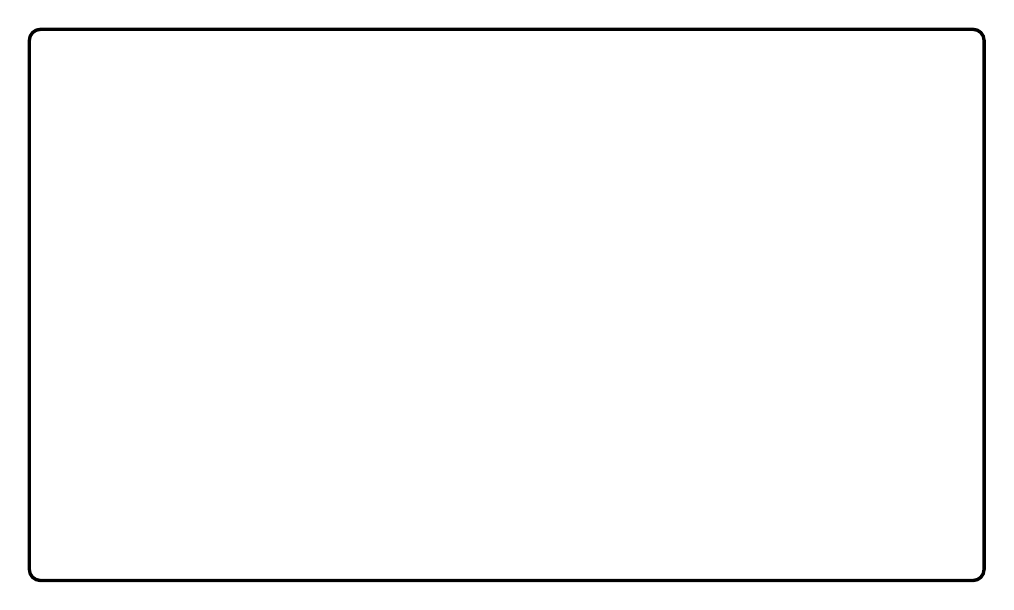
\begin{tikzpicture}
  \draw[rounded corners, line width=1.2pt] (0,0) rectangle (\linewidth,7cm);
\end{tikzpicture}
\end{center}

\bigtask{4. The most symmetric thing}
A plate or a wheel has endless fold lines. What is the most symmetric thing you
found? Draw it and one of its fold lines.

\begin{center}
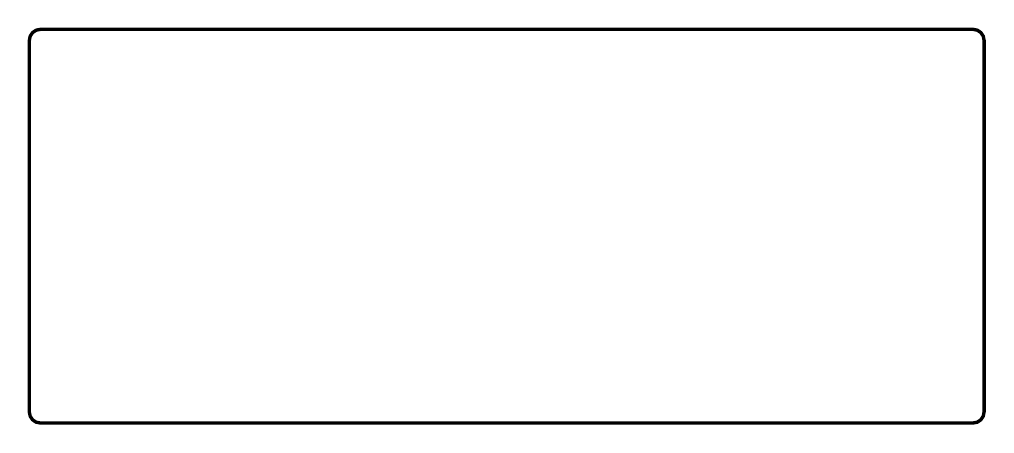
\begin{tikzpicture}
  \draw[rounded corners, line width=1.2pt] (0,0) rectangle (\linewidth,5cm);
\end{tikzpicture}
\end{center}

\end{document}
